\documentclass[10pt]{article}

\usepackage{mathtools}
\DeclarePairedDelimiter\ceil{\lceil}{\rceil}
\DeclarePairedDelimiter\floor{\lfloor}{\rfloor}


\usepackage{graphicx}
\graphicspath{{img/}}
\usepackage{amsmath}
\usepackage[margin=1.0in]{geometry}
\usepackage{hyperref}
\hypersetup{
	colorlinks=true,
	linkcolor=blue
}


\begin{document}

\title{\vspace{-2.0cm}Milestone 1 - Modeling}
\author{Neeraj Gandhi, Ramneet Kaur, Abhijeet Singh, Nikhil Shenoy}
\date{\today}

\maketitle

\section{Model Descriptions}
	In all the templates described below, x is a global clock that was declared in the “Descriptions” part of the model.

	\subsection{Heart}

		\begin{figure}[h]
			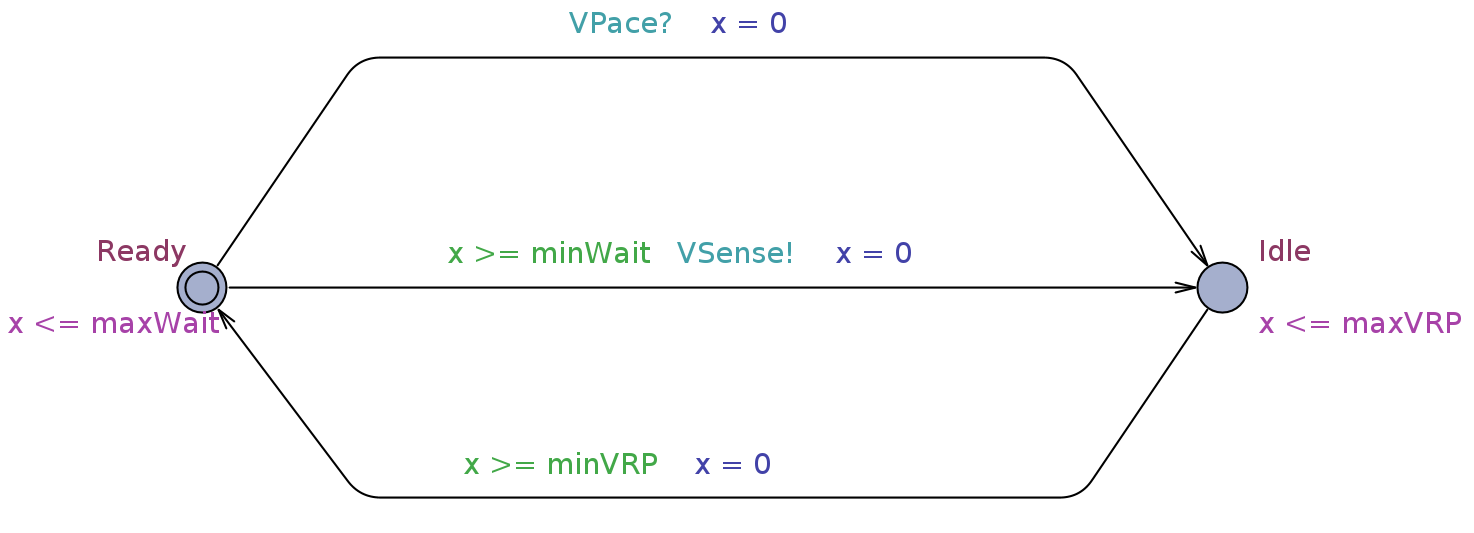
\includegraphics[scale=.35]{heart_model.jpg}
			\label{heart_model}
			\centering
			\caption{The Heart Model}
		\end{figure}

		The Heart starts out in the Ready state. The middle arrow is a transition that occurs if the Heart beats normally. The transition described by the top-most arrow occurs when the pacemaker provides a stimulus to the Heart. Finally, the state machine travels back to the state in which it expects to receive a heartbeat (either natural or artificial) when the clock x is greater than or equal to the minimum VRP and less than or equal to the maximum VRP.


	\subsection{Ventricle}
		\begin{figure}[h]
			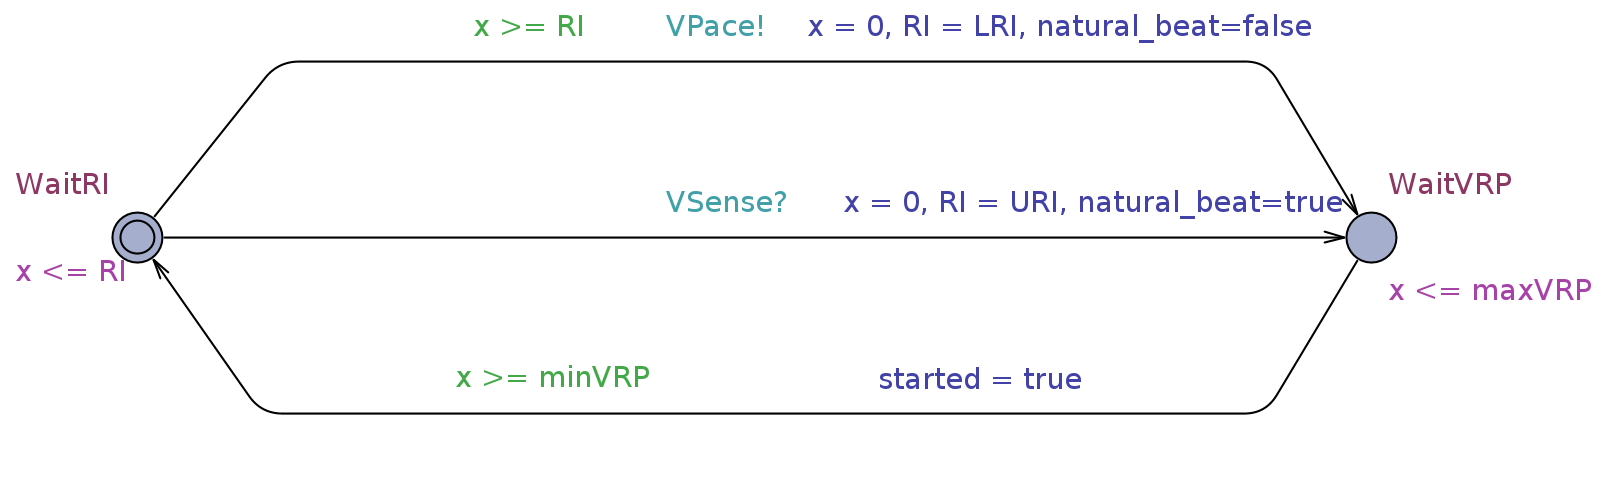
\includegraphics[scale=.35]{ventricle_model.jpg}
			\label{ventricle_model}
			\centering
			\caption{The Ventricle Model}
		\end{figure}

		The Ventricle starts in the WaitRI state. Here, it waits to sense the occurrence of a natural heartbeat within a certain time frame, and if the time bound is exceeded it sends a stimulus to the heart. The Ventricle then moves into the WaitVRP state, which is a period during which no signals can be received. Once the VRP, bounded by minVRP and maxVRP, has elapsed, the Ventricle will return to the WaitRI state and wait for Sense signals.


	\subsection{Observer}
		\begin{figure}[h]
			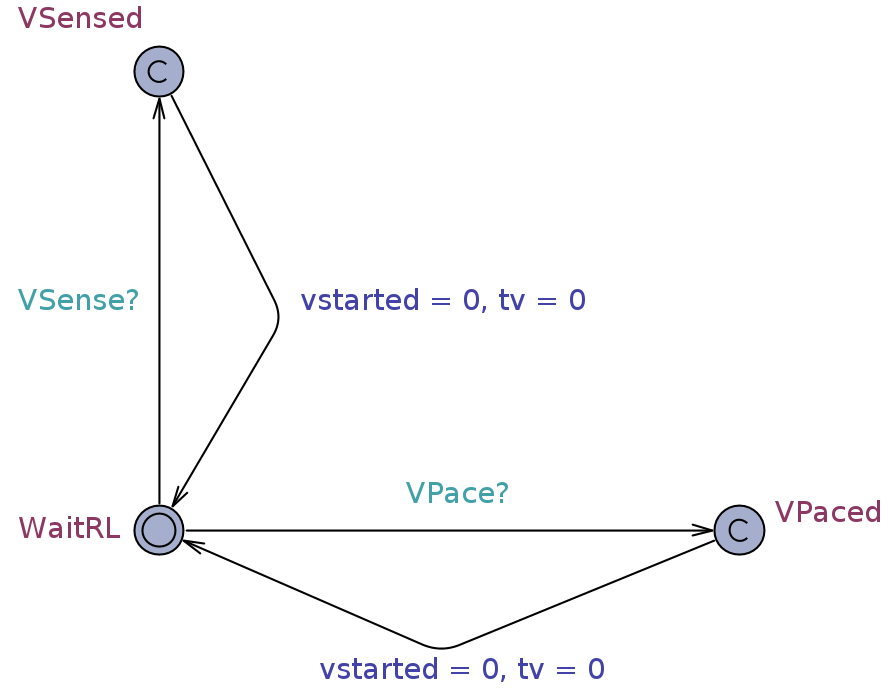
\includegraphics[scale=.35]{observer_model.jpg}
			\label{observer_model}
			\centering
			\caption{The Observer Model}
		\end{figure}

		The Observer is used to model the external monitor of the interaction between the pacemaker and the heart. The Observer simply waits for a sensed heartbeat or a simulated heartbeat, changes states, and then changes states back. In the implementation, these state transitions would likely be logged so that if a doctor or someone else wanted to assess the health of the heart they could use the frequency of simulated heartbeats as an assessment parameter.

\section{Query Descriptions}


	\subsection{A[] not deadlock}
		This is the standard deadlock query. This query makes sure that our system does not get stuck in a particular state and stop progressing.


	\subsection{A[](Ventricle.WaitVRP \&\& Heart.Idle) imply x $<=$ maxVRP}

		This query means that when both the Ventricle and Heart are in their respective waiting states (Ventricle.WaitVRP and Heart.Idle), the clock will be less than the maxVRP. By using maxVRP, we ensure that no signals are received during any possible VRP within the specification. By requiring that both Ventricle and Heart are in waiting states, we know that Sense/Pace signals will not be sent or received.

	\subsection{A[] ((Ventricle.WaitRI \&\& Ventricle.started \&\& !Ventricle.natural\_beat) imply Ventricle.RI $==$ Ventricle.LRI)}

		This query states that after sending a pacing signal to the Heart, the Pacemaker will wait(at most) for the next Lower Rate Interval. This is because it is possible that the heart beats naturally within the next Lower Rate Interval after it was paced by the Pacemaker. Pacemaker(after sending a pacing signal) should therefore wait for the longest permissible interval(which is LRI) for sensing the natural heartbeat.

	\subsection{A[] ((Ventricle.WaitRI \&\& Ventricle.started \&\& Ventricle.natural\_beat) imply Ventricle.RI $==$ Ventricle.URI)}

		This query covers the case after the Pacemaker has sensed a natural beat from the heart. It would then wait for the next Upper Rate Interval to sense the natural beat. A shorter interval can be used here because a natural heart will regularly beat in intervals faster than the Lower Rate Interval.

	\subsection{A[] ((Ventricle.WaitRI \&\& Ventricle.started) imply x $>=$ minVRP}

		This query indicates that the Ventricle is started and ready to act or react based on the behavior of the Heart. It shows that the earliest the Pacemaker can act is at the end of the shortest Ventricular Refractory Period.

\section{Acknowledgements}

	We drew from the model specified on slide 42 of ``Pacemaker Timing Cyles-F13-F17-v3.pdf'' to create this design. These slides were made available to us through Canvas.
	
\end{document}









